\documentclass[10pt]{article}

% Required Packages
\usepackage{amsmath, amssymb} % For mathematical symbols and equations
\usepackage{graphicx} % For including figures
\usepackage[utf8]{inputenc} % For UTF-8 encoding
\usepackage[T1]{fontenc} % For better font encoding
\usepackage{microtype} % For better typography
\usepackage{booktabs} % For better-looking tables
\usepackage{array} % For better table control
\usepackage{multirow} % For multi-row in tables
\usepackage[colorlinks=true, allcolors=blue]{hyperref} % For hyperlinks
\usepackage{url} % For formatting URLs
\usepackage{geometry} % For adjusting page margins
\geometry{a4paper, margin=1in} % Set margins

% Title and Author Information
\title{A Spectral Alphabet Wheel for Modeling Letter Transitions in German and English}
\author{Daniel Hommers \\
        private research \\
        \texttt{daniel@hommers.de}}
\date{} % Remove the date

\begin{document}

\maketitle

\begin{abstract}
Modeling letter/digraph transitions can reveal phonotactic structure useful for computational linguistics and language modeling. We introduce the Alphabet Wheel, a data-driven representation that places letters and key digraphs as operators on a circle via spectral embedding; in real corpora, operator flows prefer small angular turns. For German (DE, N=14 sectors) and English (EN, N=16), the wheel’s energy (mean angular turn) is significantly lower than two nulls—angle-shuffle (z $\approx$ -3.13 DE; -3.40 EN) and degree-preserving (z $\approx$ -2.51 DE; -3.79 EN)—and token placements are stable (DE: median circular SD $\approx$ 9.38$^\circ$, 97.5\% sector agreement; EN: SD $\approx$ 42.6$^\circ$ across domains). A shuffled-angle baseline shows $\sigma^\circ$ $\approx$ 114$^\circ$ and $\approx$9\% sector agreement, underscoring the effect. High-PMI ``chords'' (e.g., QU$\to$ECK, PMI=2.47) highlight language-specific constraints. The framework yields a compact, falsifiable phonotactic prior with immediate applications in NLP and linguistic visualization.
\end{abstract}

\textbf{Keywords:} phonotactics, spectral embedding, letter transitions, graph models, computational linguistics

\section{Introduction}
Local n-gram models capture short-range dependencies but miss higher-level structure. We propose the Alphabet Wheel: letters and fused digraphs act as operators placed on a circle so that typical flows take short angular steps. The wheel is learned from corpus bigrams and validated against null models. We present DE (single official corpus) and EN (news/web/wiki), with plans to extend to Indonesian.

\section{Methods}
\subsection{Data \& Tokens}
Upper-case letters; DE diacritics normalized (Ä$\to$AE, Ö$\to$OE, Ü$\to$UE, ß$\to$SS). Fused tokens as single operators (DE: SCH, CH, ST, NG, PF, QU; EN: TH, SH, PH, GH, ST, PR, \ldots). Bigrams ($C_{ij}$) built over word-internal transitions (BOS/EOS optional).

\subsection{Spectral Embedding}
Compute a 2D spectral embedding (complex eigenvector of row-stochastic $P$, or first non-trivial pair of the normalized Laplacian). Angles $\theta_i = \mathrm{atan2}(\Im v_i,\Re v_i)$; rotate so the vowel centroid $\approx$ 100$^\circ$. For EN splits, align news/web/wiki frames to NEWS by mean-phasor. For DE stability, re-embed from the symmetric graph $A=(C + C^\top)/2$.

\subsection{Mod-N Selection}
Per-edge turn $\Delta\theta_{ij} = \arccos(\cos(\theta_j - \theta_i))$. Energy $E=\sum p_{ij}\Delta\theta_{ij}$ with $p_{ij}$ proportional to counts. Quantize to $N\in\{13,14,15,16\}$ sector centers and pick $N$ by the most negative z against two nulls: (1) angle-shuffle (permute angles, fixed counts); (2) degree-preserving (IPF/Sinkhorn; fixed row/col sums).

\subsection{Viability Calculus \& H-Adapter}
Assign edge viability by PMI and turn: $\top$ if PMI $\geq$ 1.0 and $\Delta\theta \le \pi/4$; $\bot$ if PMI $<$ 0 and $\Delta\theta > 2\pi/3$; else $\sim$. The optional H-adapter upgrades $\sim \to \top$ if both $s\to H$ and $H\to d$ exist—capturing H as a consonant bridge/hinge.

\subsection{Stability Metrics}
DE: Poisson bootstrap (B=200) on counts; symmetric re-embedding; circular SD $\sigma^\circ$ and mod-14 sector agreement vs. baseline.  
EN: cross-domain circular SD after frame alignment; mod-16 sector agreement.

\subsection{Artifacts}
Reproducible CSVs (mod-N sweeps, per-token tables, stability, viability, chords):\\
\texttt{alphabet\_wheel\_min\_release\_v01.zip} 

\section{Results}
\subsection{Mod-N Selection}
DE: N=14 (z $\approx$ -3.13 angle-shuffle; -2.51 degree-preserving).  
EN: N=16 (z $\approx$ -3.40; -3.79).

\subsection{Stability (with context)}
DE (B=200): 40 tokens, median $\sigma^\circ$ $\approx$ 9.38$^\circ$ (p90 $\approx$ 17.01$^\circ$); 97.5\% sector agreement (mod-14). Shuffled-angle null: $\sigma^\circ$ $\approx$ 114$^\circ$, agreement $\approx$ 9\% ($\approx$1/14).  
EN (news/web/wiki): 43 tokens, median $\sigma^\circ$ $\approx$ 42.6$^\circ$ (p90 $\approx$ 76.7$^\circ$); 2/43 tokens fully stable (mod-16). Stable: OL ($\approx$3.4$^\circ$), ST ($\approx$9.1$^\circ$); less stable: O, B ($\approx$78–88$^\circ$).

\subsection{Operator Cards (core)}
Per-token fields: angle $\theta^\circ$, sector (mod-N), $\sigma^\circ$, onset/coda vowel shares, viability (out/in $\top$/$\sim$/$\bot$).  
DE narrative: QU acts as a clamp (very low out$\top$/in$\top$, resolves mainly before vowels, e.g., QU$\to$ECK, PMI=2.47, Section 3.4); SCH/H show high outgoing viability with large H-upgrade shares (cluster bridges); ST is permissive (out$\top$ $\approx$ 0.958) and matches ST$\gg$TS (e.g., ST$\to$ECK, PMI=2.37). See Figure~\ref{fig:de-wheel} for a visualization of the DE wheel and its key chords.

\subsection{Top Chords}
PMI-ranked chords showcase constraints. We highlight QU, ST (DE) and TH, ST (EN) for their high mass and phonotactic significance in consonant clusters and vowel transitions. Examples: DE QU$\to$ECK (PMI=2.47), ST$\to$ECK (2.37); EN TH$\to$E (1.54), Y$\to$ST (1.84).

\section{Discussion}
The wheel captures robust phonotactic structure: lower energy than nulls, stable sectors (especially DE), and interpretable operators (QU clamp; SCH/H hinges; ST ratchet/pre-closure). The DE vs. EN stability contrast ($\sigma^\circ$ $\approx$ 9.38$^\circ$ vs. 42.6$^\circ$) reflects corpus coherence: DE’s single official corpus ensures tight clustering, while EN’s news/web/wiki diversity increases angular variability. The vowel-free skeleton remains significant in DE, indicating a consonantal backbone. Applications include phonotactic priors for segmentation/decoding and error detection via large-$\Delta\theta$, low-PMI edges.

\section*{References}
\begingroup
\renewcommand{\section}[2]{} % Remove the default "References" title
\begin{thebibliography}{10}

\bibitem{vonLuxburg2007}
von Luxburg, U. (2007).
\newblock A tutorial on spectral clustering.
\newblock \textit{Statistics and Computing}, 17(4), 395–416.

\bibitem{jurafsky2021}
Jurafsky, D., \& Martin, J. H. (2021).
\newblock \textit{Speech and Language Processing} (3rd ed.).
\newblock Draft. Retrieved from \url{https://web.stanford.edu/~jurafsky/slp3/}

\bibitem{hayes2008}
Hayes, B., \& Wilson, C. (2008).
\newblock A maximum entropy model of phonotactics.
\newblock \textit{Linguistic Inquiry}, 39(3), 379–440.

\end{thebibliography}
\endgroup

\section{Conclusion}
A compact, data-driven Alphabet Wheel summarizes operator flow in DE/EN, beats strong nulls, and offers practical priors and visualizations.

\begin{figure}[htbp]
    \centering
    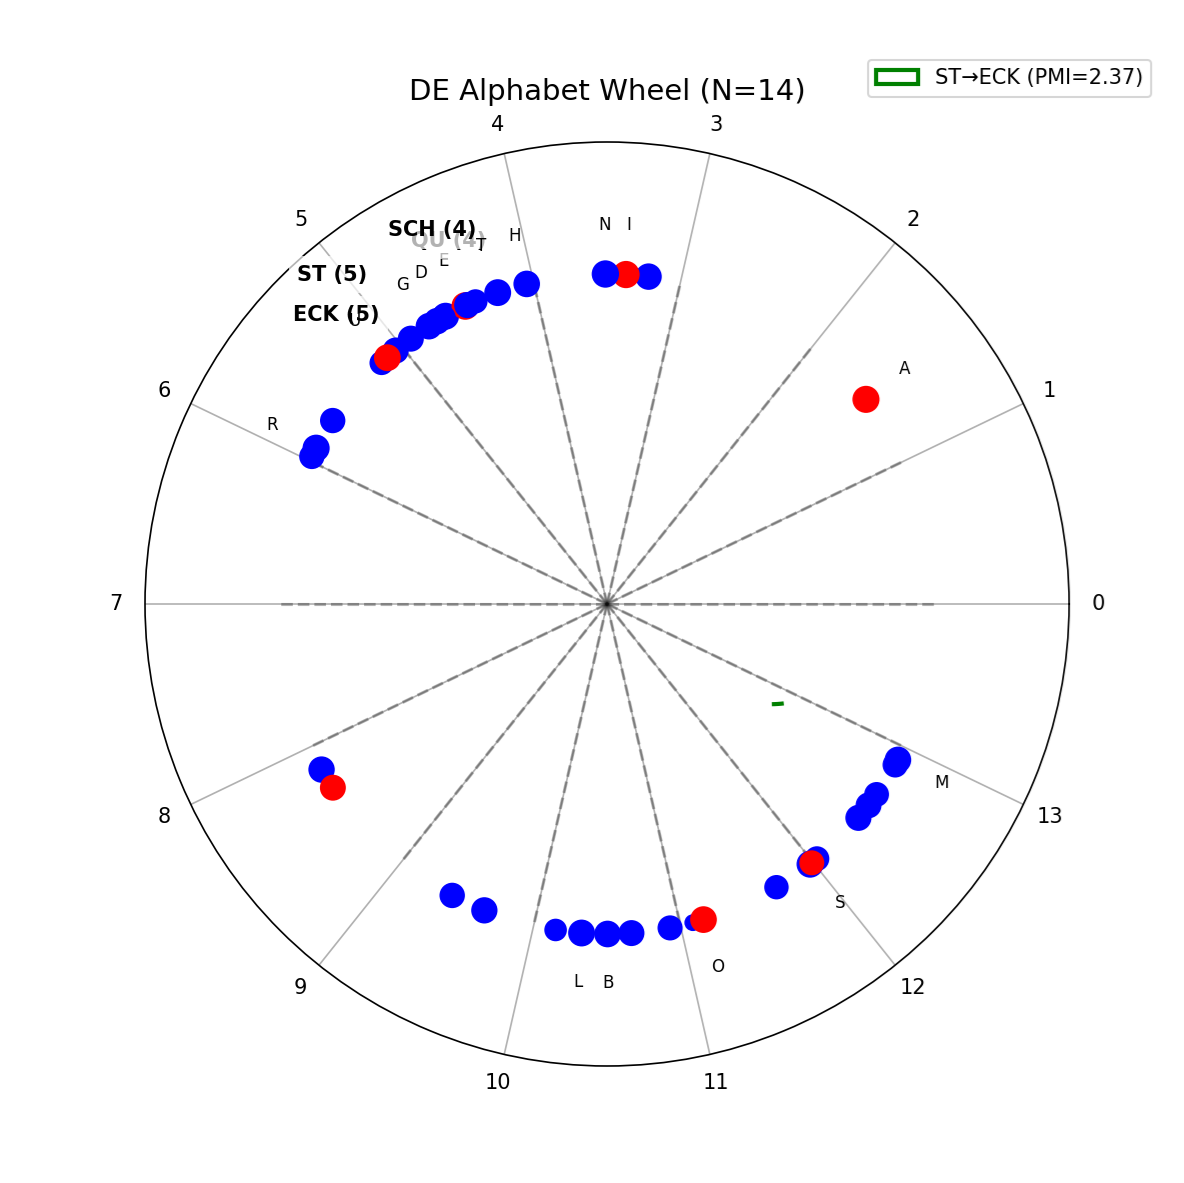
\includegraphics[width=0.8\linewidth]{de_wheel.png} % Replace with your actual figure filename
    \caption{DE Alphabet Wheel (N=14) showing key operators (QU: $\theta^\circ$ $\approx$ 113.5, SCH: $\theta^\circ$ $\approx$ 126.5, ST: $\theta^\circ$ $\approx$ 129.8) and top chords (e.g., ST$\to$ECK, PMI=2.37, $\Delta\theta$=0.06).}
    \label{fig:de-wheel}
\end{figure}

% In Section 3.3
\begin{figure}[h]
    \centering
    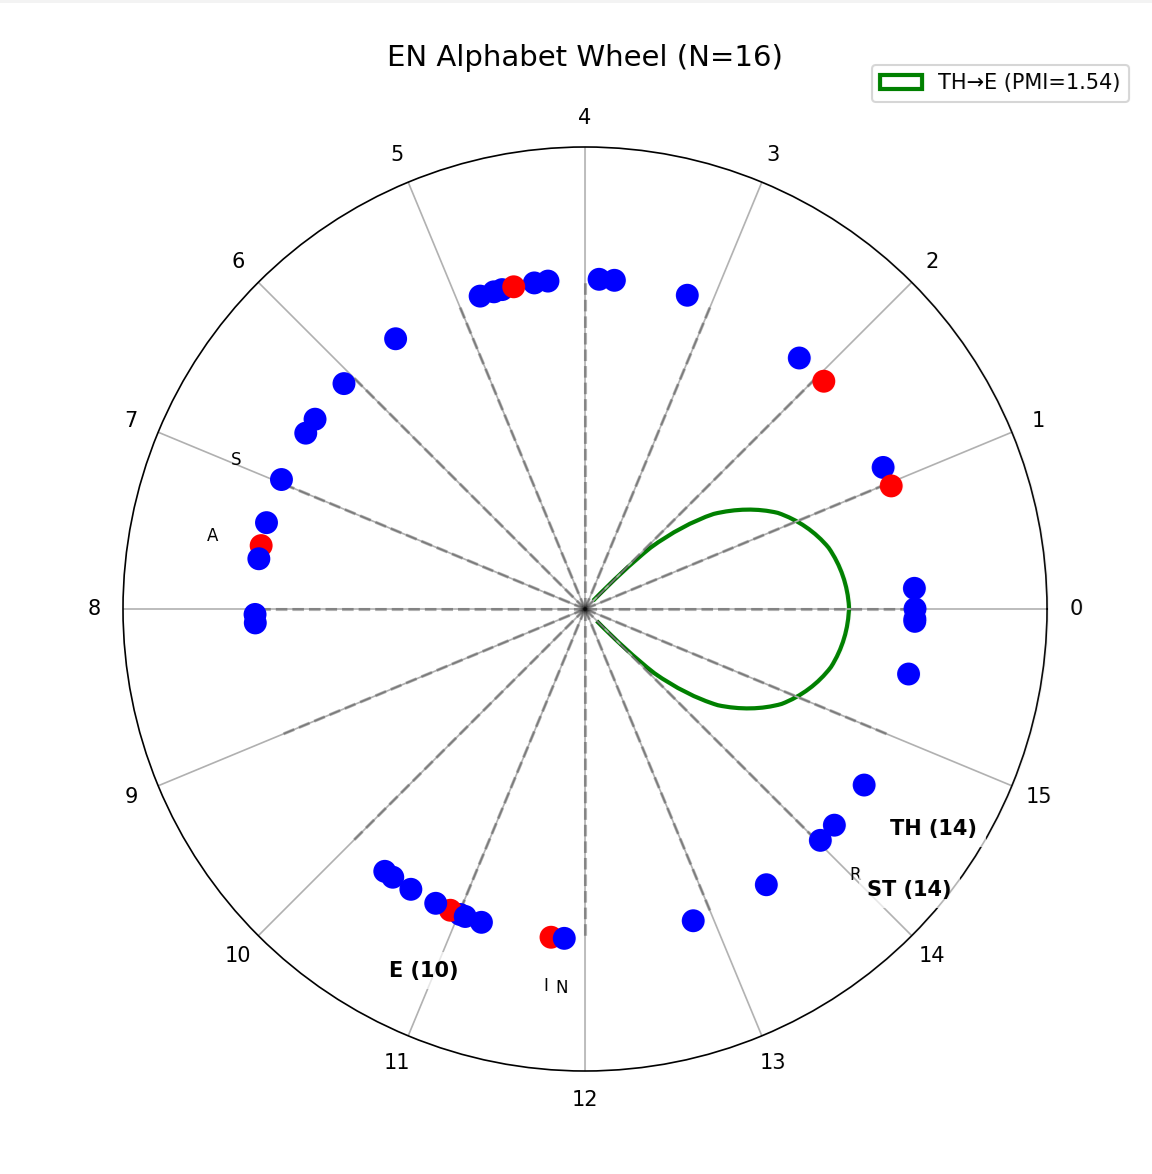
\includegraphics[width=0.5\textwidth]{en_wheel.png}
    \caption{EN Alphabet Wheel (N=16) showing key operators (TH: $\theta^\circ \approx 327.8$, ST: $\theta^\circ \approx 319.1$, E: $\theta^\circ \approx 245.9$) and top chords (e.g., TH$\to$E, PMI=1.54). Angles reported in the same frame as the figure.}
    \label{fig:en_wheel}
\end{figure}


\end{document}